\documentclass{deck}
\usepackage[american]{babel}
\usepackage{merriweather}
\usepackage{soul}
\usepackage[absolute]{textpos}\TPGrid{16}{16}\ttfamily
\definecolor{background}{HTML}{F0F5F5}\pagecolor{background}
\pagestyle{empty}
\setstretch{1.1}
\sethlcolor{zgreen}
\begin{document}
\setlength{\parindent}{0pt} % indent first line

\setlength{\fboxsep}{2pt}
\newcommand\point[2]{\vbox{\raggedright\small%
  \fcolorbox{zgreen}{white}{\color{zgreen}#1}\newline%
  \footnotesize#2\vspace{16pt}}}
\newcommand\highlight[1]{{\color{white}{\hl{\thinspace#1\thinspace}}}}

\begin{textblock}{14}[0,0](2,13){
  \setstretch{1.0}\color{gray}\footnotesize
  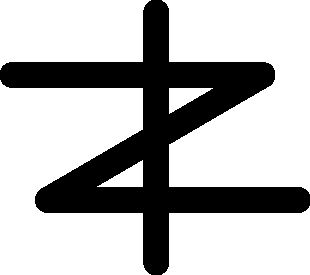
\includegraphics[height=24pt]{../images/zerocracy-logo.pdf}
  
\includegraphics[height=24pt]{../images/logo.pdf}\\
  This is not an investment offer. To get an actual SAFE,
  contact us by \href{mailto:cio@zerocracy.com}{email}.\\
  555 Bryant Str, Ste 470, Palo Alto, CA 94301, 408.692.4742\\
  \today\quad\zoldversion
}\end{textblock}

\begin{textblock}{7}[1,0](15,13){\begin{flushright}
  \setstretch{1.0}\color{gray}\footnotesize
  Media about us:\\
  \href{https://www.cio.com/article/3326560/artificial-intelligence/workplace-ai-emerging-technologies-ethical-questions.html}{
\includegraphics[height=12pt]{../images/cio-logo.pdf}}
\end{flushright}}\end{textblock}

\begin{multicols}{3}

\point{Artificial Intelligence}{
  \href{https://www.zerocracy.com}{Zerocracy} is an AI-empowered chatbot that
  helps project managers coordinate programmers, increasing the quality and decreasing costs.
  The uniquiness is in the pay-by-result management \href{https://www.xdsd.org}{model} we invented in 2009, which
  \highlight{revolutionary} disrupts the market, leading the fast-growing trend of
  \href{http://papers.zold.io/freelance-deck.pdf}{freelancing}.
  Read more about our \href{http://papers.zold.io/zerocracy-deck.pdf}{mission},
  \href{http://papers.zold.io/features-deck.pdf}{features}
  and \href{http://papers.zold.io/arc-deck.pdf}{architecture}.}

\point{Cryptocurrency}{
  \href{https://www.zold.io}{Zold} is a non-Blockchain cryptocurrency for fast
  micropayments, invented and created by \href{https://www.yegor256.com/about-me.html}{Yegor Bugayenko},
  the CEO and founder of Zerocracy. As its \href{http://papers.zold.io/green-paper.pdf}{Green Paper}
  explains, Zold is way faster than any other
  existing cryptocurrency, including Bitcoin and Ethereum, and much
  cheaper in maintenance. The \href{http://papers.zold.io/wp.pdf}{White Paper} fully discloses the details
  of the invented technology. \highlight{8\%} of Zold total capacity is
  owned by Zerocracy.}

\point{RPA Market}{
  According to the \href{http://www.transparencymarketresearch.com/it-robotic-automation-market.html}{recent report}
  of Transparency Market Research, ``automation is soon expected
  to become a game changing technology in the transformation of IT industry.''
  Zerocracy is the \highlight{first} and \highlight{unique} player that automates
  project management.}

\point{Traction}{
  The chatbot has been in the R\&D phase since August 2016.
  It's met its first paying customers in May 2018.
  At the moment, there are 300+ programmers registered,
  five paying clients, and \highlight{\$15K+} monthly revenue.
  To get more details, \href{mailto:is@zerocracy.com}{subscribe} to our monthly investor snapshot.}

\point{Crypto Traction}{
  The R\&D of the cryptocurrency has been started in February 2018.
  The first payment has been sent on May 27, 2018. Since than
  there were over 20K payments sent and over 5K wallets registered
  by over a thousand users.}

\point{Team}{
  There are \href{http://papers.zold.io/zerocracy-deck.pdf}{seven people},
  including software engineers, AI experts,
  and investment advisers in Zerocracy/Zold team. The team works together
  for the last two years and is going to double its size in the next year.}

\point{Visibility}{
  The community that supports the idea of Zerocracy and Zold includes
  thousands of software enthusiasts, in our \href{https://blog.zold.io}{two}
  \href{https://www.zerocracy.com/blog.html}{blogs},
  \href{https://t.me/zerocracy}{two} \href{https://t.me/zold_io}{groups} in Telegram,
  \href{https://twitter.com/0crat}{Twitter}, and \href{https://facebook.com/zerocracy}{Facebook}.}

\point{Targets}{
  Our target clients are 40K+ software companies worldwide, which
  eventually will realize that full-time employment is the past, while
  pay-by-result and
  \href{http://papers.zold.io/freelance-deck.pdf}{freelance} is the future. The revenue expected
  to achieve in the next ten years is \highlight{\$400M}
  with \highlight{80\%} profit margin.
  More details can be found in the \href{http://papers.zold.io/executive-summary.pdf}{Executive Summary}.}

\point{Fund Raising}{
  \$850K+ has been invested into Zerocracy by its founders so far.
  At the moment it is seeking investments in amount of \highlight{\$1.6M} in exchange for
  \href{https://en.wikipedia.org/wiki/Simple_agreement_for_future_equity_(SAFE)}{SAFE notes}
  with pre-money cap of \highlight{\$16M}.
  The minimum amount is \$100K.
  USD, BTC, and ETH accepted.}

\point{Expenses}{
  The funds will be spent on
    programming and source code maintenance (30\% of the budget),
    research \& development (20\%);
    market visibility (20\%);
    business development (10\%);
    investors relationship and further fundraising (10\%);
    legal support (10\%).}

\point{Exit}{
  It is predicted that the valuation of Zerocracy will grow \highlight{10x} in the next
  two years, thanks to the market expansion and Zold emission. The ultimate
  objective is IPO in 5-6 years with the valuation of \$4B, which means
  \highlight{250x} for first-round investors.}

\end{multicols}

\end{document}
